% Project Specifications

\chapter{The Generator Model}

\section{A Description of GANs}

There are two networks in a GANs model: $D$, the discriminator, and $G$, the generator. $D$ is a regular
classifier which models a function $f: X -> P$ where $X$ are the input examples and $P$ is the probability
that $x \in X$ came from real training data rather than data generated by $G$. In a sense, this probability
value identifies the input example as "authentic" or not, so the higher the probability, the better $D$ does
at discriminating authentic data against data "faked" by $G$. $G$, on the other hand, trys to fool $D$ by
generating output that resembles the real data, and learns the probability distribution during the training
process. If the learning is successful, $G$ will be able to create new samples from the distribution it
has learned.

% The task of $D$ is to learn to correctly label both types of examples. Meanwhile, $G$ learns to
% generate examples that mimic real world examples.

During the training, we feed two types of examples to $D$: existing training examples and examples generated
by $G$. The system can be trained with regular stochastic gradient descent and backpropagation. The training
process improves the ability of both $D$ and $G$, until eventually the output of $G$ will be
indistinguishable from real world examples to $D$. Once trained, $D$ can be discarded and $G$ can be used
in different applications.

In the original paper both networks are multilayer perceptrons, however many different network types have been
proposed since then. In this project, $D$ and $G$ are both deep convolutional neural networks which are
suitable for image processing. The training of $D$ and $G$ is done on GPU with floating-point numbers. Since
$D$ is discarded after training, from now on we are only concerned with $G$.

\section{DCGAN Network Structure}

\begin{figure}[h]
  \centering
  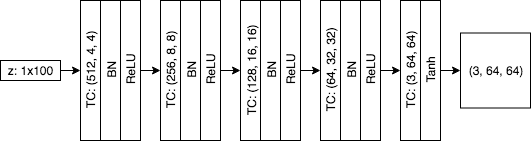
\includegraphics[scale=0.5]{network_structure}
  \caption{DCGAN Network Structure}
  \label{fig:network_structure}
\end{figure}

\ref{fig:network_structure} shows the network structure of $G$, with five transposed convolutional layers.
Except for the last transposed convolutional layer, the previous four transposed convolutional layers each
are followed by a layer of batch normalization, and a layer of rectified linear units (ReLU) for
activation. The last transposed convolutional layer is followed by a layer of $tanh$ function applied to
each element as activation. The parameters for each layer is detailed in \ref{table:network_layers}.
The network structure is rather simple compared with many other much larger networks. ResNet, for example,
contains a deep cascade of 152 layers.

\begin{table}[h]
  \centering
  \caption{DCGAN Layers}
  \begin{tabular}{l | l | l }
    \toprule
    Layer & Type & Description \\
    \midrule
    1 & TC & $100 \rightarrow 512$ channels, $4 \times 4$ kernel, stride $1$, padding $0$ \\
    2 & BN & $512$ channels\\
    3 & ReLU & $512$ channels \\
    4 & TC & $512 \rightarrow 256$ channels, $4 \times 4$ kernel, stride $2$, padding $1$ \\
    5 & BN & $256$ channels \\
    6 & ReLU & $256$ channels \\
    7 & TC & $256 \rightarrow 128$ channels, $4 \times 4$ kernel, stride $2$, padding $1$ \\
    8 & BN & $128$ channels \\
    9 & ReLU & $128$ channels \\
    10 & TC & $128 \rightarrow 64$ channels, $4 \times 4$ kernel, stride $2$, padding $1$ \\
    11 & BN & $64$ channels \\
    12 & ReLU & $64$ channels \\
    13 & TC & $64 \rightarrow 3$ channels, $4 \times 4$ kernel, stride $2$, padding $1$ \\
    14 & Tanh & 3 channels, final layer \\
    \bottomrule
  \end{tabular}
  \label{table:network_layers}
\end{table}

\clearpage %force the next chapter to start on a new page. Keep that as the last line of your chapter!
